\documentclass[12pt,twoside,a4paper]{article}
\usepackage{amssymb}
%\usepackage{fullpage}
\usepackage[T1]{fontenc}
\usepackage[latin1]{inputenc}
\usepackage[french]{babel}
\usepackage{array} % and/or
\usepackage{longtable} % and/or
%\usepackage{colortab} % or
\usepackage{colortbl}
\usepackage{arydshln}
%\usepackage{wasysym}
\usepackage{txfonts}
\usepackage{textcomp}
\usepackage{graphicx}
\usepackage{multicol}
\usepackage{numprint}
\usepackage[usenames, dvipsnames]{xcolor}
\usepackage{tikz}
%\usetikzlibrary{shapes.geometric}
%\usetikzlibrary{shapes.multipart}
\usepackage{enumitem}
\usepackage{minitoc}


\everymath{\displaystyle}
\begin{document}

\linespread{1,5} %Interligne 1,5
\thispagestyle{empty} %Cette commande sert à enlever la pagination sur la page titre
\begin{center} % Centre le texte
\textbf{Les Bourbaki} \\
\vspace{5 cm}
Pr\'esent� par\\
Florence Duperr� et Alexandra Gobeil \\
\vspace{5 cm}
Travail pr�sent� dans le cadre du cours de\\
Histoire de la math�matique\\
\vspace{5 cm}
\today 
\end{center} %Arrêter de centrer le texte
\newpage %Nouvelle page


\setcounter{page}{1} %On demande de compter les pages à partir d'ici à la page 1
\tableofcontents %Ajoute la table des matière

\newpage  %Nouvelle page

%\listoffigures %Ajoute la table des images (vous pouvez l'enlever pour les travaux courts)

\newpage
\section{Introduction}
\section{Historique}
\subsection{Avant guerre}
\subsection{Pendant guerre}
\subsubsection{La l�gende du nom Nicolas Bourbaki}
Le pr�nom Nicolas Bourbaki provient d'un g�n�ral de l'arm�e du 19�me si�cle qui n'a rien � voir avec les math�matiques. Ils auraient choisi ce nom pour deux raisons. La premi�re serait en honneur � ce g�n�ral qui a �t� important dans la guerre franco-prussienne.La deuxi�me est due � une blague qui a �t� faite � l'�cole normale sup�rieure, comme quoi le g�n�ral Bourbaki allait venir parler de math�matique d'une fa�on particuli�re. 
\\

L'un des avantages d'avoir choisi ce pr�nom est qu'il rend la soci�t� encore plus myst�rieuse et les rend plus intrigants, ce qui permet de les faire connaitre davantage. 
\newpage
\subsection{Apr�s guerre}
\subsection{Influence aujourd'hui}
\section{La ruse des Bourbaki}
\begin{center}
	
	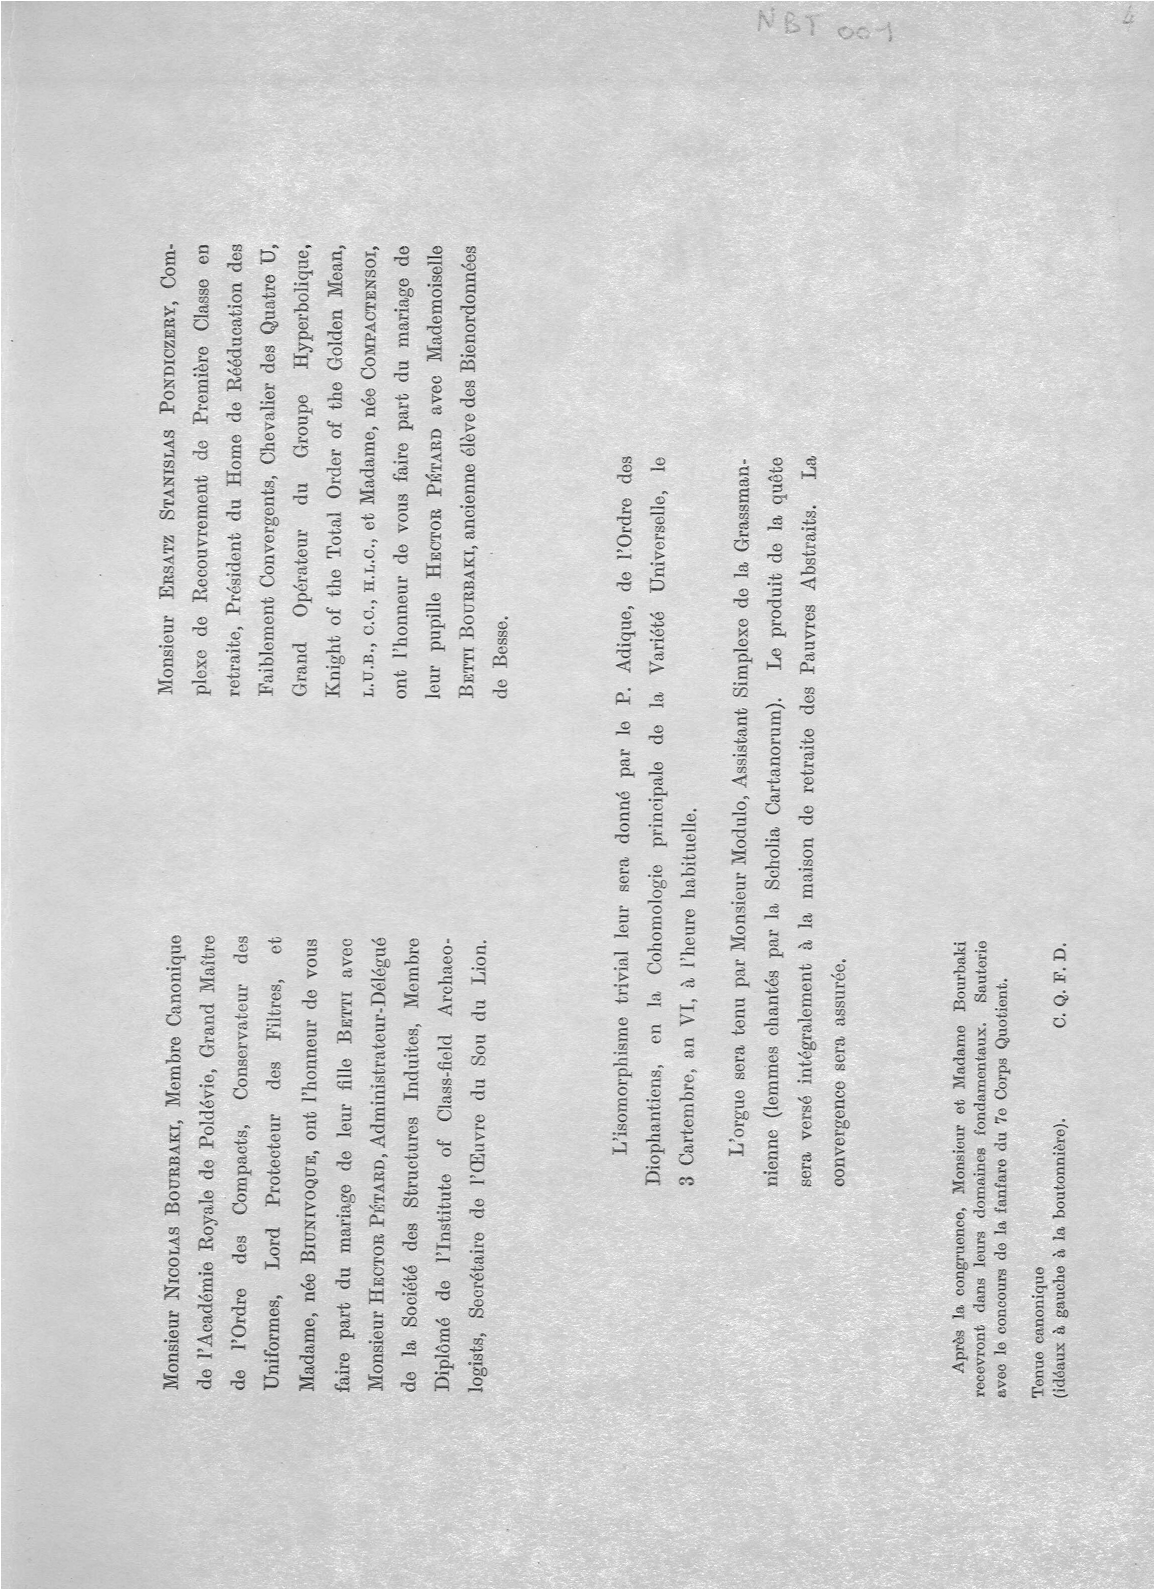
\includegraphics[scale=0.4,angle=270]{marriage.png}
\end{center}
\end{document}